\documentclass{article}
\usepackage{amsmath}
\usepackage{amssymb}
\usepackage{geometry}
\usepackage{array}
\usepackage{mathtools}
\usepackage{tikz}
\geometry{a4paper, margin=1in}

\begin{document}

\title{Résumé Complet sur les Matrices avec Exemples et Illustrations}
\author{Issam}
\date{}
\maketitle

\tableofcontents
\newpage

%------------------------------------------
\section{Définition générale}
Une matrice $A \in \mathbb{R}^{m \times n}$ est un tableau rectangulaire de nombres :
\[
A = \begin{pmatrix}
a_{11} & a_{12} & \cdots & a_{1n} \\
a_{21} & a_{22} & \cdots & a_{2n} \\
\vdots & \vdots & \ddots & \vdots \\
a_{m1} & a_{m2} & \cdots & a_{mn}
\end{pmatrix}
\]

%------------------------------------------
\section{Types de matrices}

\begin{center}
\begin{tabular}{|c|c|c|}
\hline
Type & Forme générale & Propriétés principales \\
\hline
Carrée & $n \times n$ & diagonale, inverse possible si $\det \neq 0$ \\
\hline
Diagonale & $d_i$ sur diagonale & $A^T = A$, multiplication facile \\
\hline
Identité & 1 sur diagonale & $AI = IA = A$ \\
\hline
Nulle & 0 partout & $0+A = A$, $0\cdot A = 0$ \\
\hline
Symétrique & $A = A^T$ & valeurs propres réelles \\
\hline
Triangulaire & $a_{ij}=0$ au-dessus ou en dessous & $\det = \prod d_i$ \\
\hline
Orthogonale & $A^T A = I$ & $A^{-1} = A^T$ \\
\hline
\end{tabular}
\end{center}

\subsection*{Exemple graphique d'une matrice $3 \times 3$}
\begin{center}
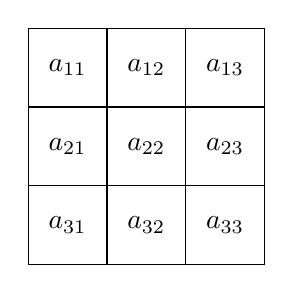
\begin{tikzpicture}
\draw (0,0) rectangle (3,3);
\foreach \x in {0,1,2} {
    \foreach \y in {0,1,2} {
        \draw (\x,\y) rectangle (\x+1,\y+1);
    }
}
\node at (0.5,2.5) {$a_{11}$};
\node at (1.5,2.5) {$a_{12}$};
\node at (2.5,2.5) {$a_{13}$};
\node at (0.5,1.5) {$a_{21}$};
\node at (1.5,1.5) {$a_{22}$};
\node at (2.5,1.5) {$a_{23}$};
\node at (0.5,0.5) {$a_{31}$};
\node at (1.5,0.5) {$a_{32}$};
\node at (2.5,0.5) {$a_{33}$};
\end{tikzpicture}
\end{center}

%------------------------------------------
\section{Opérations sur les matrices}

\subsection{Addition}
\[
A + B = (a_{ij} + b_{ij})
\]

\textbf{Exemple :}
\[
A = \begin{pmatrix}1 & 2\\ 3 & 4\end{pmatrix}, \quad
B = \begin{pmatrix}5 & 6\\ 7 & 8\end{pmatrix} \quad \Rightarrow \quad
A+B = \begin{pmatrix}6 & 8\\ 10 & 12\end{pmatrix}
\]

\subsection{Multiplication}
\[
C = AB, \quad c_{ij} = \sum_{k=1}^{n} a_{ik}b_{kj}
\]

\textbf{Exemple :}
\[
A = \begin{pmatrix}1 & 2\\ 0 & 1\end{pmatrix}, \quad
B = \begin{pmatrix}3 & 0\\ 1 & 2\end{pmatrix}
\]
\[
AB = \begin{pmatrix}1\cdot3 + 2\cdot1 & 1\cdot0 + 2\cdot2 \\ 0\cdot3 + 1\cdot1 & 0\cdot0 + 1\cdot2\end{pmatrix}
= \begin{pmatrix}5 & 4 \\ 1 & 2\end{pmatrix}
\]

\subsection{Transpose}
\[
A^T = (a_{ji})
\]

\textbf{Exemple :}
\[
A = \begin{pmatrix}1 & 2 & 3\\ 4 & 5 & 6\end{pmatrix} \quad \Rightarrow \quad
A^T = \begin{pmatrix}1 & 4\\ 2 & 5\\ 3 & 6\end{pmatrix}
\]

%------------------------------------------
\section{Déterminant et Inverse}

\subsection{Cas $2\times2$}
\[
A = \begin{pmatrix}a & b\\ c & d\end{pmatrix} \quad \Rightarrow \quad
\det(A) = ad-bc
\]

\textbf{Exemple :}
\[
A = \begin{pmatrix}2 & 3\\ 1 & 4\end{pmatrix} \quad \Rightarrow \quad
\det(A) = 2\cdot 4 - 3\cdot 1 = 5
\]

\subsection{Inverse}
\[
A^{-1} = \frac{1}{\det(A)} \begin{pmatrix}d & -b\\ -c & a\end{pmatrix}
\]

\textbf{Exemple :}
\[
A^{-1} = \frac{1}{5} \begin{pmatrix}4 & -3\\ -1 & 2\end{pmatrix} = \begin{pmatrix}0.8 & -0.6\\ -0.2 & 0.4\end{pmatrix}
\]

%------------------------------------------
\section{Rang d'une matrice}
\[
\text{rang}(A) = \text{nombre de lignes non nulles après réduction}
\]

\textbf{Exemple :}
\[
A = \begin{pmatrix}1 & 2 & 3\\ 2 & 4 & 6\\ 0 & 1 & 1\end{pmatrix} 
\quad \Rightarrow \text{réduction} \quad
\begin{pmatrix}1 & 2 & 3\\ 0 & 0 & 0\\ 0 & 1 & 1\end{pmatrix} \quad \Rightarrow \text{rang}=2
\]

%------------------------------------------
\section{Systèmes linéaires}

\[
Ax = b
\]

\textbf{Exemple :}
\[
\begin{pmatrix}2 & 1\\ 1 & 3\end{pmatrix} \begin{pmatrix}x\\y\end{pmatrix} = \begin{pmatrix}5\\6\end{pmatrix}
\quad \Rightarrow \quad x=1, y=2
\]

%------------------------------------------
\section{Valeurs propres et vecteurs propres}

\textbf{Exemple :}
\[
A = \begin{pmatrix}2 & 1\\ 1 & 2\end{pmatrix}
\]
\[
\det(A-\lambda I) = \begin{vmatrix}2-\lambda & 1\\1 & 2-\lambda\end{vmatrix} = (2-\lambda)^2 - 1 = 0
\]
\[
\lambda_1 = 1, \quad \lambda_2 = 3
\]

Vecteurs propres :
\[
v_1 = \begin{pmatrix}1\\ -1\end{pmatrix}, \quad v_2 = \begin{pmatrix}1\\1\end{pmatrix}
\]

%------------------------------------------
\section{Diagonalisation}
\[
A = PDP^{-1}, \quad P = \text{vecteurs propres}, \quad D = \text{valeurs propres diagonale}
\]

\textbf{Exemple :}
\[
P = \begin{pmatrix}1 & 1\\ -1 & 1\end{pmatrix}, \quad
D = \begin{pmatrix}1 & 0\\ 0 & 3\end{pmatrix}
\]

%------------------------------------------
\section{Décomposition SVD}
\[
A = U \Sigma V^T
\]

\textbf{Exemple :}
\[
A = \begin{pmatrix}3 & 0\\ 4 & 5\end{pmatrix} \quad \Rightarrow \text{SVD: } U,\Sigma,V^T
\]

\begin{center}
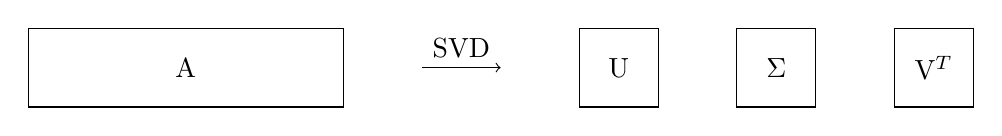
\begin{tikzpicture}
\draw (0,0) rectangle (4,1) node[pos=.5] {A};
\draw[->] (5,0.5) -- (6,0.5) node[midway,above] {SVD};
\draw (7,0) rectangle (8,1) node[pos=.5] {U};
\draw (9,0) rectangle (10,1) node[pos=.5] {$\Sigma$};
\draw (11,0) rectangle (12,1) node[pos=.5] {V$^T$};
\end{tikzpicture}
\end{center}

\end{document}
